\documentclass{beamer}
\beamertemplatenavigationsymbolsempty
\usepackage{amsmath, amssymb, hyperref, graphics, tikz}
%\usepackage{mathpazo, soul}



\newcommand{\C}{\mathbb{C}}
\newcommand{\Z}{\mathbb{Z}}
\newcommand{\R}{\mathbb{R}}
\newcommand{\N}{\mathbb{N}}
\DeclareMathOperator{\Real}{Re}
\DeclareMathOperator{\Imag}{Im}


\title{Complex Analysis MAS332 \\ Lecture 1}
\author{Paul Johnson \\ \href{mailto:paul.johnson@sheffield.ac.uk}{paul.johnson@sheffield.ac.uk} \\ Office: Hicks J06b}
\date{October 1st}

\begin{document}

\maketitle

  \begin{frame}{Complex Analysis: What's all this, then?}
 Up until now: derivatives and integrals of functions $f:\R^n\to \R^m$

 \begin{block}{Derivatives and integrals of $f:\C\to\C$}
     \begin{itemize}
     \item Easier than real case!
     \item Analysis not a prerequisite -- not focused on \emph{doing} proofs
     \item \emph{Using} theorems correctly, building on each other
     \end{itemize}
 \end{block}
 
   \begin{theorem}[Fundamental Theorem of Algebra] Let $p(z)\in \C[x]$ be a nonconstant polynomial.  Then there is a $w\in\C$ with $p(w)=0$.
\end{theorem}

\begin{block}{The Residue Theorem has bonkers applications:}   
     $$\int_{-\infty}^\infty \frac{\cos(\pi x)}{(1+x^2)^2}dx=\frac{\pi}{2}e^{-\pi}(\pi+1)$$
\end{block}
 

  
  \end{frame}

    \begin{frame}[plain]
        \begin{tikzpicture}[remember picture,overlay]
            \node[at=(current page.center)] {
                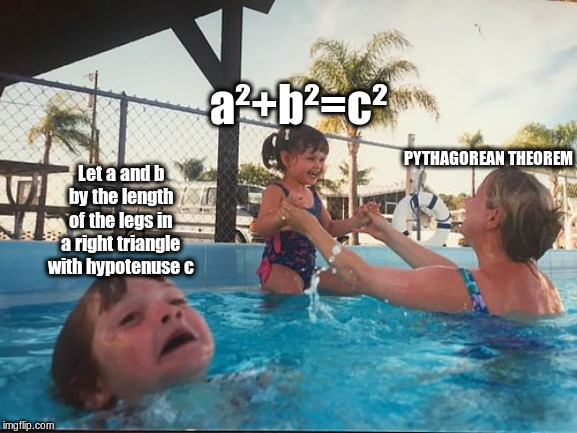
\includegraphics[keepaspectratio,
                                 width=\paperwidth,
                                 height=\paperheight]{PythagorasMeme.jpg}
            };
        \end{tikzpicture}
     \end{frame}



\begin{frame}{Written Resources}
\begin{block}{Main resource: Dr. Hart's notes}
\begin{itemize}
\item  Fine-tuned toward the exam
\item Many worked examples
\end{itemize}
\end{block}

\begin{block}{Recommended texts: extra material + viewpoints, more rigour}
\begin{itemize}
\item Priestley (pdf through library)
\item Stewart and Tall (old edition is cheap online)
\end{itemize}
\end{block}

\begin{block}{Slides}
\begin{itemize}
\item Posted online before lecture; space to write notes
\item Roughly follow Dr. Hart's notes
\end{itemize}
\end{block}
\end{frame}

\begin{frame}{Assessment and feedback}
  \begin{block}{100\% of marks from final exam}
\begin{itemize}
\item Exam questions generally very similar to past years
\item \alert{Four mandatory questions this year instead of five}
  \item Forthcoming exam page will have more detail
\end{itemize}
  \end{block}
  \begin{block}{Exercises and feedback}
    \begin{itemize}
    \item Exercise and hints sheets on MOLE -- \alert{DO DURING TERM}
    \item Will collect a few to mark for feedback
    \item Worked solutions to all exercises will go up shortly after that
            \end{itemize}
  \end{block}
  \begin{block}{Interactive ``clicker questions'' in lecture}
\begin{itemize}
\item    Using TurningPoint app/webpage 
\item Everyone gets instant feedback on how things are going
\end{itemize}
\end{block}
\end{frame}

\begin{frame}[plain,c]

\begin{center}

\Huge

\usebeamercolor[fg]{frametitle}
Clicker Session \\
\\
Turning Point app or:
\\
ttpoll.edu 

\end{center}





\end{frame}

\begin{frame}{Review of complex numbers}
  The complex plane $\C=\{z: z=x+iy; x,y\in\R\}$.
  \begin{itemize}
  \item $x=\text{Re}(z)$ is called the \emph{real part} 
  \item $y=\text{Im}(z)$ is called the \emph{imaginary part} 
  \item $\overline{z}=x-iy$ is called the \emph{complex conjugate} 
  \item $|z|=\sqrt{x^2+y^2}$ is called the \emph{modulus} of $z$

  \end{itemize}
  \begin{block}{Complex numbers form a field}
Can add, multiple, subtract by any complex number, and divide by nonzero complex numbers.
\end{block}

\end{frame}

\begin{frame}{A few tricks}
  \begin{block}{$\C\cong\R^2$}
    An equation $z=w$ of complex numbers can be viewed as a pair of equations between real numbers:
$$z=w \iff  \Real(z)=\text{Re}(w) \text{ and } \Imag(z)=\Imag(w)$$
  \end{block}

  \begin{block}{Why care about $\overline{z}$?}
    $$|z|^2=z\cdot \overline{z}$$
    This lets us find $z^{-1}$.
\end{block}
  \begin{example}What's $\frac{1-i}{3+4i}$?

    \end{example}

\end{frame}

\begin{frame}{Geometry of complex numbers}
  \begin{theorem}[Euler]
    $$e^{i\theta}=\cos(\theta)+i\sin(\theta)$$
  \end{theorem}
  \begin{block}{Polar form / ``modulus-argument'' form}
  If we write $z=x+iy$ in polar coordinates:
  $$z=r\cos(\theta)+ir\sin(\theta)=r e^{i\theta}$$
\end{block}
  \begin{block}{Multiplying and dividing easier in polar form!}
  $$(re^{i\theta})(se^{i\phi})=(rs)e^{i(\theta+\phi)}$$
  $$\frac{re^{i\theta}}{se^{i\phi}}=(r/s)e^{i(\theta-\phi)}$$
  \end{block}
  \end{frame}
\begin{frame}{Powers and roots}
  \begin{theorem}[De Moivre] Let $\theta\in\R$ and $n\in \Z$.  Then
    $$(\cos\theta+i\sin\theta)^n=\cos n\theta+i\sin n\theta$$
  \end{theorem}
  \begin{proof} Apply Euler's theorem to both sides of $(e^{i\theta})^n=e^{in\theta}$, or prove directly for $n\in \N$ using induction and trig formulas.   \end{proof}
  
   \begin{theorem}
    A complex number $z=re^{i\theta}$ has precisely $n$ $n$th roots:
    $$\sqrt[\leftroot{-2}\uproot{2}n]{r}e^{i(\theta+2k\pi)/n} \quad \quad k\in\{0,1,\dots,n-1\}$$
    \end{theorem}


\end{frame}

\end{document}
